\section{Algorithms}
\label{Sect:Algo}

{\bf Lead author:} Adam

\subsection{General Code Structure}

MAUS operates on data using distinct modules which fall into four types: input, output, map and reduce. Input modules take data from a source and read into memory e.g. offline DAQ data, JSON files, etc. Output send data to file, e.g. ROOT or JSON. Maps perform the main work on the data, and must not perform any kind of data persistency spill to spill. Reducers are then used when it is required to accumulate data over multiple spills, e.g. to produce histograms in real time.  

A diagram showing the tracker software data flow with the corresponding modules is shown in figure~\ref{Fig:DataFlow}.

\begin{figure}[htb]
    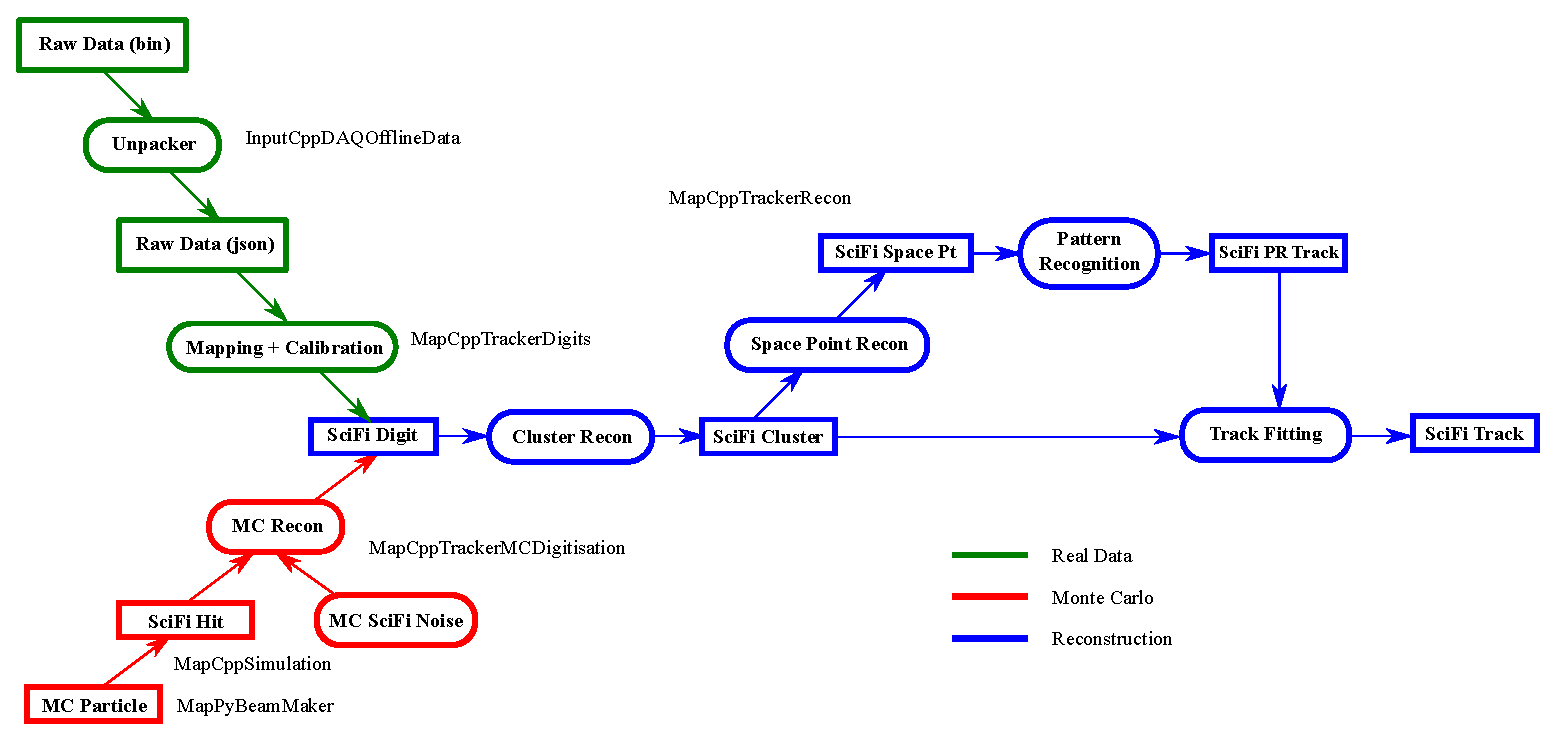
\includegraphics[width=1.0\textwidth]
      {06-Algorithms/Figures/DataFlow.eps}
    \caption{Schematic of the tracker software data showing MC and Real data input, and subsequent reconstruction. MAUS modules corresponding to given process are indicated (MapCppTrackerRecon encompasses all of the reconstruction, shown in blue).  Once digits have been formed, reconstruction is agnostic as to whether the MC or Real path was followed.}
    \label{Fig:DataFlow}
\end{figure}

